% Author: Aadarsha Paudel
% Use it for anything you want.
% PS: You don't need to edit this file, go edit contents in
% files/ folder. That file has everything you need to modify.

\documentclass[a4paper,12pt]{report}
\usepackage{calc} % does some calculation
\usepackage[utf8]{inputenc} % modern fonts and utf8 support
%\usepackage{times} % times new roman text
\usepackage[vmargin=1in,hmargin=1in]{geometry} % margin to 1 inch
\usepackage{titlesec} % change section title format
\usepackage{graphicx} % for images
\usepackage[font=small,labelfont=bf]{caption} % image caption
\usepackage[nomain,acronym]{glossaries} % for abbreviations
\usepackage{setspace} % normal spacing
\usepackage{parskip} % paragraph spacing
\usepackage{diagbox} % for diagonal line in time schedule table
\usepackage[table]{xcolor} % for colors (black in chart)
\usepackage{pgfgantt} % gantt chart (for time schedule)


% Some Quick Formatting for Glossary Page (List of Abbreviation)

\newglossarystyle{mylist}{%
\renewcommand*{\glossentry}[2]{%
\item[\glsentryitem{##1}%
\glstarget{##1}{\glossentryname{##1}}]

\glossentrydesc{##1} \glspostdescription }%
}

\setglossarystyle{mylist}
\makeglossaries

\newacronym{php}{PHP}{PHP Hypertext Preprocessor}
\newacronym{css}{CSS}{Cascading Style Sheets}
\newacronym{js}{JS}{JavaScript}
\newacronym{html}{HTML}{Hypertext Markup Language}

 % importing abbreviations


\setlength{\parindent}{15pt} % space after paragraph


\def\figurename{\textbf{Figure }}

\renewcommand{\Huge}{\fontsize{14}{14}} % Huge font size
\renewcommand{\arraystretch}{1.5} % better table row height

\titleformat{\chapter}[block]
{\normalfont%
    \Huge
    \bfseries}{\thechapter}{14pt}{
    \Huge
    \uppercase
    }

\titleformat{\section}{\fontsize{12}{12}\bfseries}{\thesection}{0.5em}{\uppercase}
\titleformat{\subsection}{\fontsize{12}{12}\bfseries}{\thesection}{0.5em}{\uppercase}

\renewcommand{\contentsname}{\fontsize{14}{14}\centering\MakeUppercase{Table of Contents}}
\renewcommand{\listfigurename}{\fontsize{14}{14}\centering\MakeUppercase{List of Figures}}
\renewcommand{\listtablename}{\fontsize{14}{14}\centering\MakeUppercase{List of Tables}}
\renewcommand{\bibname}{\fontsize{14}{14}\centering\MakeUppercase{References}}

\newcommand{\cen}{\centering}
\begin{document}

% ----------------------
% 		INDEX (COVER) FILE
% ----------------------

% As the file name says, this is for the title page.
% Campus logo is at images/ folder, go replace that if you are from different Campus
% Also, change the "YOUR PROJECT NAME" on below as well as your and your friend's name and symbol number.
% Also chage the campus's name and location if you are from different campus
% Thats all for this page. If you want custom date, there is a \today at the bottom of this file, change it to any date you want (Type it manually like: June 5, 2019 or something to let others believe that you completed this report many days ago)


\begin{titlepage}
\topskip0pt
\vspace*{\fill}
\begin{centering}

    \begin{spacing}{2}
    \textbf{\Huge\uppercase{Affiliated Tribhuwan University}}


    \textbf{\Huge\uppercase{Institute of Science and Technology}}


    \textbf{\Huge\uppercase{Lumbini ICT Campus}}
    
    \vspace{15pt}
    \begin{figure}[ht!]
        \centering
        
\includegraphics[height=100pt]{images/logo}
    \end{figure}


    \end{spacing}
    
    \begin{spacing}{1.8}
    \textbf{A Project Proposal on}
    \\

    % ----------------------------------
    % CHANGE YOUR TOPIC NAME BELOW
    % ----------------------------------

    \textbf{\Huge{YOUR TOPIC NAME}}
    
    \end{spacing}

    \begin{spacing}{1.3}
        A report submitted for the partial fulfillment of requirements for the degree of Bachelor of Science in Computer Science and Information Technology.
    \end{spacing}

    \vspace{10pt}

\begin{spacing}{1.3}
\textbf{Submitted By}


Aadarsha Paudel (SYMBOL_NO/074)

Name of Your Friend (SYMBOL_NO/074)

Name of Your Friend (SYMBOL_NO/074)

% Please leave a blank line after the name to let it create new paragraph, else it will show all weird

\end{spacing}

\vspace{10pt}

\begin{spacing}{1.3}
    
    \textbf{Submitted To}

    LUMBINI ICT CAMPUS


    GAINDAKOT, NAWALPUR 

\end{spacing}
\vspace{10pt}

% -------------------------------------
% Hey, change the below line for custom date

\today

\end{centering}
\thispagestyle{empty}
\vspace*{\fill}
\end{titlepage}

\newpage

% Set Left Justify Text
% \raggedleft
% ----------------------
% 		Acknowledgement
% ----------------------
\setcounter{page}{1}
\renewcommand{\thepage}{\Roman{page}}

\chapter*{\centering{Acknowledgement}}
\addcontentsline{toc}{chapter}{Acknowledgement}
PUT YOUR ACKNOWLEDGEMENT STUFFS HERE.

\\
\\
\noindent
Aadarsha Paudel (SYMBOL_NO/074)         $\rule{3cm}{0.15mm}$ \\
\\
Name of Your Friend (SYMBOL_NO/074)         $\rule{3cm}{0.15mm}$ \\
\\
Another Friend (SYMBOL_NO/074)         $\rule{3cm}{0.15mm}$ \\
\\

\newpage

\chapter*{\centering{Abstract}}
\addcontentsline{toc}{chapter}{Abstract}
PUT YOUR ABSTRACT HERE.
\newpage

\tableofcontents % Table of Contents
\newpage
\listoffigures % List of Figures
\addcontentsline{toc}{chapter}{List of Figures}

\listoftables % List of Tables
\addcontentsline{toc}{chapter}{List of Tables}

%\chapter*{\centering{List of Abbreviation}}

\printglossary[type=\acronymtype, title=\fontsize{14}{14}\centering{\MakeUppercase{List of Abbreviation}}, toctitle=List of Abbreviation]
\addcontentsline{toc}{chapter}{List of Abbreviation}

\pagebreak

%\addcontentsline{toc}{chapter}{\listfigurename}
\setcounter{page}{1}
\renewcommand{\thepage}{\arabic{page}}


\chapter{Introduction}
\section{Background}

Background about your project.


\section{Objectives}

Why are you working on this project.

\section{Applications}

Is it useful anywhere or is it another new "blockchain" technology? Where will it apply in real life scenario? Describe here.


\section{Purposed System}

\begin{figure}[ht!]
    \centering
    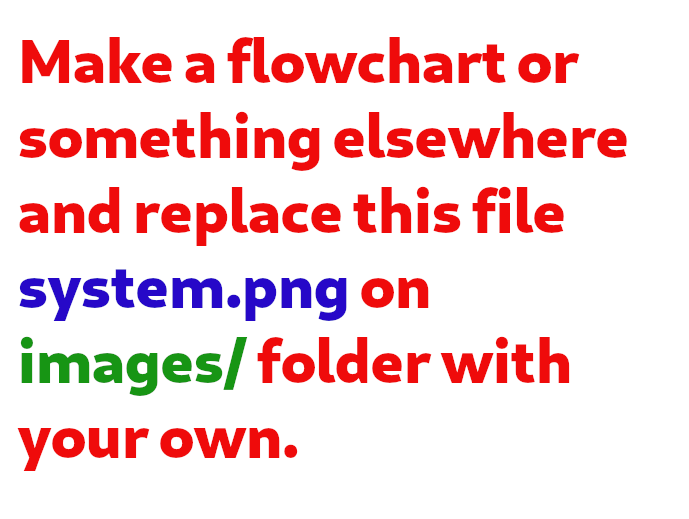
\includegraphics[width=\textwidth]{images/system}
    \caption{Purposed System \label{overflow}}
\end{figure}

\noindent
In above figure of our purposed system, we have highlighted the connection and data flow in our barebone system.


\section{Problems and Limitations}

Will your project have limitations? Bugs? Of course, it has. Describe about them here in detailed manner and how you are working on minimizing those limitations or give valid reasons about how you cant fix those.


\newpage

\chapter{Literature Review}
\section{Significance of Study}

The main purpose of your project. What will it achieve? Describe here, better write it on bullets (lists). Use 
\begin{itemize}

\item First Item

\item Second Item

\end{itemize}


\section{Related Works}

Is your project unique on its own? Probably not. Describe about other projects similar to yours and how you are different from them (on how you are better, not how you are worse than older works)


\chapter{Methodology}
\section{Data Collection}
Do you need to collect data for this project? How will you do it? Describe. You can remove if you don't need this section.

\section{Algorithm}

This will be the basic algorithm for the book suggestion:

\noindent
Step 1: Start\\
Step 2: Something Something\\
Step 3: Another thing you do\\
Step 4: End

% It is better to put double backslash (\) on above than creating new paragraph.

\section{System Overview}
What technologies you are gonna use? Like programming language, database servers, frontend, backend, all sorts of stuffs.

Better use subsection.

% Usage:
% \subsection*{TOPIC_NAME}
%
% Remove the % infront and change the TOPIC_NAME to what you want to describe like, if its PHP, use:
% \subsection*{PHP} and on next line start describing a bit about it.
% The * after subsection means it will not show up in table of contents.
% If you want to show it in table of contents, remove *, duh.


\section{Testing and Debugging Tools}

These are the list of tools that we will use for testing and debugging our programs.

Use subsection as above for better formatting.


\section{Cost Estimation}


The cost estimation of the project is as follows:

\begin{table}[h!]
\begin{center}
\begin{tabular}{ | m{0.1\textwidth} | m{0.7\textwidth}| m{0.2\textwidth} | } 
\hline
1& Proposal Printing & NPR 100  \\ 
\hline
2& Report with Hard Copy Binding & NPR 800 \\ 
\hline
3& Miscellanous & NPR 100 \\ 
\hline
& \textbf{Total} & \textbf{NPR 1000} \\ 
\hline
\end{tabular}
\caption{Cost Estimation}
\label{table:1}
\end{center}
\end{table}



\chapter{Time Schedule}
\section{Gantt Chart}

% Hello everyone, I spent a day making this chart and finding what went wrong when xcolor gave weird errors, so don't say its ugly okay, thanks.
%
% Search for gantt chart examples if you want something else.
% You can customize it if you want, learn yourself.
% PS: Most Documentation on internet are outdated and won't compile.
% This one works btw. I tried it. I worked on it so hard.
% 


Here is the gantt chart for the time schedule for this project.

\vspace{10pt}
\begin{table}[h!]
\begin{centering}
\begin{ganttchart}[
    hgrid,
    vgrid,
    x unit=100pt,
    bar height = 1, %necessary to make it fit the height
    title height = 1,
    bar top shift = 1, %to move it inside the grid space ;)
    ]{1}{3}
    \gantttitle{Week 1}{1}
    \gantttitle{Week 2}{1}
    \gantttitle{Week 3}{1}
    \ganttbar[bar/.append style={fill=black}]{Project Proposal}{1}{1}\\
    \ganttbar[bar/.append style={fill=black}]{Project Development}{1}{2}\\
    \ganttbar[bar/.append style={fill=black}]{Project Testing}{3}{3}\\
    \ganttbar[bar/.append style={fill=black}]{Documentation}{2}{3}\\
\end{ganttchart}
\caption{Time Schedule}
\label{table:2}

\end{centering}
\end{table}


\chapter{Conclusion}
\section{Expected Result}

STUFFS TO PUT HERE.

\section{Further Improvements}

WRITE SOMETHING HERE TOO.


\medskip
 
\begin{thebibliography}{9}

\bibitem{id}
Author_Name, Work_Name \textit{(Retrieved June 8, 2019)}
\\\texttt{LINK_TO_THE_WEBSITE}

% If you want to reference and show little wikipedia like [1], [2] indexing on the cited area use \cite{id}
% -------
% Please replace the id on above
% You can remove \\\texttt{} if you don't have website to reference.
% You can make it your formatting, search for biblatex on internet.
% Customize how you want, its up to you.
%

\end{thebibliography}
\addcontentsline{toc}{chapter}{References}



\end{document}

% End of document mate
% nothing beyond here